\ifdefined\included
\else
\documentclass[a4paper,11pt,twoside]{StyleThese}
\include{formatAndDefs}
\sloppy
\begin{document}
\setcounter{chapter}{-1} %% Num�ro du chapitre pr�c�dent ;)
\dominitoc
\dominilof
\faketableofcontents
\fakelistoffigures
\fi

\chapter*{Introduction}
\label{chap:introduction}
\addstarredchapter{Introduction} %Sinon cela n'apparait pas dans la table des mati�res
\setcounter{secnumdepth}{-1}
\chaptermark{Introduction}

\cleardoublepage

\section*{Context and \koroibot\ project}

\begin{figure}[ht]
\centering
\includegraphics[width=0.8\linewidth]{figures/koroibot/components.png}
\caption{Graphical representation of the scientific approach of the \koroibot\ project.}
\label{fig:koroibot:components}
\end{figure}

\subsection*{Context}

This thesis has been written in the context of the European project \koroibot\ (\url{http://www.koroibot.eu/}).
The goal of the \koroibot\ project is to enhance the ability of humanoid robots to walk in a dynamic and versatile way, and to bring them closer to human capabilities.
As depicted in Fig.~\ref{fig:koroibot:components}, the \koroibot\ project partners have to study human motions and use this knowledge to control humanoid robots via optimal control methods.
Human motions are recorded with motion capture systems and stored in an open source data bank which can be found at \url{https://koroibot-motion-database.humanoids.kit.edu/}.
With these data several possibilities are exploited.
Assuming that humans minimize some criteria we can use inverse optimal control methods to find those criteria.
Walking alphabet and learning method \cite{Mandery2016b} are also used to transfer human behaviors to robots.
Finally, optimal control is used to build controllers that can eventually use these learned human behaviors while ensuring the robot safety.
Research and innovation works in \koroibot\ mainly target novel motion control methods for existing hardware.
It also derives optimized design principles for next robot generations.

\subsection*{\koroibot\ and robot challenges}

\begin{figure}
  \includegraphics[width=\linewidth]{figures/KoroibotChallengeEnhanced.pdf}
  \begin{tikzpicture}[remember picture, overlay]
    %\draw[help lines] (0,0) grid (20,10);
    %\node at (0,0) {(0,0)};
    \draw[line width=1.5pt, color=red](2.5,2) ellipse (0.8cm and .6cm);
    \draw[line width=1.5pt, color=red](5.2,1.9) ellipse (1.1cm and .6cm);
    \draw[line width=1.5pt, color=red](11.5,1.9) ellipse (1.1cm and .6cm);
    \draw[line width=1.5pt, color=red](11,4) ellipse (1.1cm and .8cm);
    \draw[line width=1.5pt, color=red](5.6,4) ellipse (1.1cm and .8cm);
    \draw[line width=1.5pt, color=red](8.2,4.2) circle (1.0cm);
  \end{tikzpicture}
  \caption{Challenges of the \koroibot\ project. In red the challenges chosen by the LAAS-CNRS.}
  \label{fig:koroibot:scheme}
\end{figure}

In addition to this ambitious scientific aspect of the project, there is an important technical component.
Following the blue line in Fig.~\ref{fig:koroibot:scheme}, the different challenges of the project are to make humanoid robots:
\begin{list}{ \arabic{point}.}{%
		\usecounter{point}%
		\setlength{\topsep}{5pt}%
		\setlength{\itemsep}{0pt}%
		\setlength{\parsep}{0pt}%
		\setlength{\labelwidth}{3.em}%
		\setlength{\leftmargin}{2em}%
		\setlength{\labelsep}{0.5em}%
	}
\item[\bluesquare] walking on a flat ground,
\item[\bluesquare] walking on an uneven ground,
\item[\bluesquare] walking on a mattress,
\item[\bluesquare] walking on a beam with/without handrail,
\item[\bluesquare] walking on a seesaw with/without handrail,
\item[\bluesquare] climbing a stair case with/without handrail,
\item[\bluesquare] walking on stepping stones,
\item[\bluesquare] going down a stair case with/without handrail,
\item[\bluesquare] and walking through a door.
\end{list}
All the team owning a robot has to perform some of these challenges.
In Fig.~\ref{fig:koroibot:robots} we can see all the robot hosted by different partners.
Ideally, the algorithms developed in the frame of the \koroibot\ project has to be integrated on all the robots.
In practice the partners chose parts of the challenge to be realized on their different robotic platforms

\begin{figure}[ht]
\centering
\includegraphics[width=0.7\linewidth]{figures/koroibot/situations_v2.png}
\caption{List of the humanoid robot used in the \koroibot\ project.}
\label{fig:koroibot:robots}
\end{figure}

\subsection*{\koroibot\ Key Performance Indicator (KPI)}

In the European project \koroibot\ we need to evaluate the improvement in terms of robot control and human likeness.
In this context and in collaboration with the H2R project, a detailed set of key performance indicators (KPI) have been proposed \cite{torricelli2015benchmarking}.
These KPI try to capture all the bipedal locomotion patterns.

A set of specific sub-function of the global motor behavior is analyzed (see Fig.~\ref{fig:koroibot:test}).
The different sub-function are divided in two.
First, the sub-function associated to body posture task with no locomotion.
And second the same sub-function but including the robot body transport.
The initial condition may vary depending on the experiment to perform.
This is the idea of the intertrial variability.
For example standing still on a horizontal flat surface is easy to reproduce at will.
Hence there is no intertrial variability.
On the contrary, while doing push recovery, it is difficult to reproduce the exact same push several times.
The sub-function are also classified taking into account the changes in the environment or not.

Each of these functions can be evaluated for different robots using the criteria depicted in Fig.~\ref{fig:koroibot:performance}.
The performance are classified in two sub categories, quantitative performance and human likeness.
In addition there are indications on the last two columns if the criteria is applicable on a standing task or on a locomotion task.

All the partners owning a humanoid robot need to perform an evaluation of these KPI.
However some movement are not possible yet on some robots of the consortium.
Hence, the different team picked meaningful criteria considering the current state of their robot and controllers.

\begin{figure}
\centering
\includegraphics[width=0.9\linewidth]{figures/koroibot/KPIexperiment.jpg}
\begin{tikzpicture}[remember picture, overlay]
    %\draw[help lines, color=blue] (-8,0) grid (8,25);
    %\node [color=red] at (0,0) {\textbf (0,0)};
    %\node [color=red] at (0,20) {\textbf (0,20)};
    %\node [color=red] at (0,10) {\textbf (0,10)};
    \draw[line width=1.5pt, color=red](-3.9,19.7) ellipse (2cm and .5cm);
    \draw[line width=1.5pt, color=red](-3.9,16.9) ellipse (2cm and .5cm);
    \draw[line width=1.5pt, color=red](-3.9,9.0) ellipse (2cm and .5cm);
    \draw[line width=1.5pt, color=red](-9.5,7.25) ellipse (2cm and .5cm);
  \end{tikzpicture}
\caption{ The motor skills considered in the benchmarking scheme. This scheme is limited to bipedal locomotion skills. The concept of intertrial variability is
analogous to the concept of unexpected disturbances.
}
\label{fig:koroibot:test}
\end{figure}

\begin{figure}
\centering
\includegraphics[width=0.90\linewidth]{figures/koroibot/KPIabilities.jpg}
\begin{tikzpicture}[remember picture, overlay]
    %\draw[help lines, color=blue] (-8,0) grid (8,25);
    %\node [color=red] at (0,0) {\textbf (0,0)};
    %\node [color=red] at (0,20) {\textbf (0,20)};
    %\node [color=red] at (0,10) {\textbf (0,10)};
    \draw[line width=1.5pt, color=red](-4.6,16.2) ellipse (2.2cm and .43cm);
    \draw[line width=1.5pt, color=red](-4.6,13.3) ellipse (2.2cm and .43cm);
    \draw[line width=1.5pt, color=red](-4.6,12.45) ellipse (2.2cm and .43cm);
  \end{tikzpicture}
\caption{The motor abilities and related benchmarks are classified in two categories: performance and human likeness. The
performance category includes all those abilities related to stability (ability of maintaining equilibrium) and efficiency. The human
likeness category includes all those abilities related to typical human behavior, under the perspective of kinematics and dynamics.
For each ability, a specific benchmark has been identified. The last column specifies in what classes of motor skills (i.e., the function
category of Fig.~\ref{fig:koroibot:test}) the corresponding benchmark is applicable.
}
\label{fig:koroibot:performance}
\end{figure}

\subsection*{The work done in the \koroibot\ context}

In LAAS-CNRS, the Gepetto team own the HRP-2 and the Romeo robots depicted respectively as the second and fourth robot in Fig.~\ref{fig:koroibot:robots} from the left to the right.
The Romeo robot is the first human size prototype of Softbank Robotics and has very limited locomotion capabilities.
Therefore I was in charge of integrating our algorithms on the HRP-2 robot.
Among the challenges from Fig.~\ref{fig:koroibot:scheme} we picked the one with a red circle, i.e:
\begin{list}{ \arabic{point}.}{%
		\usecounter{point}%
		\setlength{\topsep}{5pt}%
		\setlength{\itemsep}{0pt}%
		\setlength{\parsep}{0pt}%
		\setlength{\labelwidth}{3.em}%
		\setlength{\leftmargin}{2em}%
		\setlength{\labelsep}{0.5em}%
	}
\item[\bluesquare] walking on a flat ground,
\item[\bluesquare] walking on an uneven ground,
\item[\bluesquare] walking on a beam with/without handrail,
\item[\bluesquare] climbing a stair case with/without handrail,
\item[\bluesquare] walking on stepping stones,
\item[\bluesquare] and going down a stair case with/without handrail.
\end{list}
In addition to those challenges we added the perturbation rejection.
At the beginning of the project we evaluated the KPI on the HRP-2 robot.
In our case, we picked the KPI sub-functions meaningful considering the above selected challenges:
\begin{list}{ \arabic{point}.}{%
		\usecounter{point}%
		\setlength{\topsep}{5pt}%
		\setlength{\itemsep}{0pt}%
		\setlength{\parsep}{0pt}%
		\setlength{\labelwidth}{3.em}%
		\setlength{\leftmargin}{2em}%
		\setlength{\labelsep}{0.5em}%
	}
\item[\bluesquare] horizontal ground at constant speed,
\item[\bluesquare] stairs,
\item[\bluesquare] soft terrain with constant compliance,
\item[\bluesquare] bearing constant weight (the robot's own weight).
\end{list}
Coupled with the following benchmarks:
\begin{list}{ \arabic{point}.}{%
		\usecounter{point}%
		\setlength{\topsep}{5pt}%
		\setlength{\itemsep}{0pt}%
		\setlength{\parsep}{0pt}%
		\setlength{\labelwidth}{3.em}%
		\setlength{\leftmargin}{2em}%
		\setlength{\labelsep}{0.5em}%
	}
\item[\bluesquare] success rate across N different trials,
\item[\bluesquare] specific energy cost of transport,
\item[\bluesquare] specific mechanical cost of transport,
\end{list}
All these choices are shown in the tables from Fig.~\ref{fig:koroibot:test} and Fig.~\ref{fig:koroibot:performance} by red ellipses.
The mathematical details and results are presented below in section {"\koroibot\ Key Performance Indicator (KPI)"}.

\paragraph*{Reactive walking}
The results pointed out some interesting points.
First the ground walking velocity and versatility of HRP-2 can be improved.
In this context we did a collaboration, presented in Chap.~\ref{chap:nmpc}, with our mathematician colleagues from the University of Heidelberg.
This collaboration leads to a new real time walking pattern generator with increased functionalities like obstacle avoidance.
In addition to this, the implementation of the dynamic filter, presented by Nishiwaki and al. in \cite{Nishiwaki:IJRR:09}, increase the range of the reachable CoM velocity.
\paragraph*{Multicontact motion generation}
The second problem that arose from the KPI was the energy consumption during the stair climbing.
One possible way for solving this problem is to distribute the robot weight over multiple contacts.
Hence, we designed an innovative multi-contact controller to allow generic locomotion and the use of a handrail.
Chap.~\ref{chap:multicontact} explains this contribution in details.
\paragraph*{Fire hose manipulation}
The second application concerns perturbation rejection and has been done in a collaboration with the Japanese national institute of Advanced Industrial Science and Technology (AIST).
This application is inspired from the DARPA robotic challenge.
The idea of this work is to see if a humanoid robot with average power and size like HRP-2 is able, using a state of the art controller, to pull a stiff fire hose.
The details of the experiment are written in Chap.~\ref{chap:hose}
\paragraph*{One third power law}
In the frame of the \koroibot\ project, researchers studied the human motion to extract quantitative data.
In fact they noticed that humans adapt their velocities in function of the curvature of their trajectories.
The scientific question that we tried to answer is the following: "Can this law extracted from human motion help humanoid robots to walk ?" 
A fruitful collaboration with these experts allowed us to answer this question.
This resulted in the design of an innovating controller for tracking cyclic trajectories of the center of mass.
Chap.~\ref{chap:powerlaw} present this work in details.
\paragraph*{Human motion primitives and model predictive control}
Another collaboration with human motion experts was done to study if motion primitives extracted from human behavior could be applied to humanoid robot.
To answer this question we propose a whole body controller using upper body movement primitives extracted from human behavior and lower body movement computed by a walking pattern generator.
Chap.~\ref{chap:primitives} show these fused bottom up and top down approaches.
\paragraph*{Reactive controllers}
In this thesis we studied reactive behavior for humanoid robot.
We designed applications that make the robot facing real case scenarios.
The first application was done in the frame of a collaboration with Airbus/Future of Aircraft Factory.
The idea was to build controllers for test case scenarios and evaluate if humanoid robot could go in a factory.
We used online planner for obstacle avoidance, visual servoing coupled with a walking pattern generator to place the robot in a desired position, a whole body controller for screwing tasks, and center of pressure based walking pattern generator to climb stairs.
Chap.~\ref{chap:univworker} explains this contribution in details.


\section*{Problem statement and state of the art}

\section*{Problem Statement}
\label{sec:locomotion}

Robot behavior realization can be formalized using mathematical optimization.
Considering a robot with $N$ degrees of freedom, $\bm q$ a vector of information on its internal parameters and the environment ${\bm v} \in \mathcal{R}^m$.
For a given behavior let us assume that it exists a function
$f({\bm q},{\bm v},t):\mathcal{R}^{n \times m+1} \rightarrow [0,1]$
such as it is equal to $0$ when the behavior is realized.
The problem amount to find a trajectory ${\bm q}(t)$ such that
\begin{align}
\label{eq:optimization:generic}
\text{minimize}   &\quad f({\bm q},{\bm v},t) \\
\text{subject to} &\quad
g({\bm q},{\bm v},t) < 0 \nonumber \\
&\quad h({\bm q},{\bm v},t) = 0 \nonumber
\end{align}
with $g$ being unilateral constraint an h bilateral constraints.

A common approach in robotics is to build an approximation $\hat{f}$ of $f$.
It depends on the estimated current state of the environment $\hat{v}(t)$, and an estimation of the current state of the robot in this environment $\hat{q}(t)$.
The formulations of $\hat{v}(t)$ and $\hat{q}(t)$ are injected in \eqref{eq:optimization:generic} to solve the optimization problem.
In this document we will not address the problem of building $\hat{v}$ but assume that an appropriate software module is providing the necessary information. Therefore we will assume that a geometric description of the environment is available, and that a system is able to give a sufficiently accurate position of the robot in this environment. Practically this is done through a motion capture system.
In the following we will present the formulation of \eqref{eq:optimization:generic} for the locomotion problem.

\subsection*{The locomotion generic optimal control problem}

The state of the problem $\bm x$ is usually composed of the robot whole body configuration coupled with the whole body velocity.
Let us now denote by $\mq$ the whole body configuration and by $\mdq$ the whole body velocity.
The future contact point can be precomputed by a planner or included in the state of the problem.
The control of this system $\bm u$, can be the next derivative of the state, i.e $\mddq$, or the contact wrench $\bm\phi = \begin{bmatrix}
{\bf f}_k &
\bm{\tau}_k
\end{bmatrix}^T$ with $k \in \{0,\hdots,K\}$, $K$ being the number of contact.
Or the motor torques $\mbf{T}$.
We denote by $\underline{\bm x}$ and $\underline{\bm u}$ the state and control trajectories.

The main idea here is to be able to compute joint trajectories satisfying the general equation of the dynamics, the initial and terminal constraints, and keeping balance.
The following optimal control problem (OCP) represents a generic form of the locomotion problem:
\begin{subequations} \label{eq:ocpgen}
\begin{eqnarray}
\hspace{-3em}	\underset{\substack{\hspace{0.2em} \underline{\bm x}, \; \underline{\bm u}} }{\min } \ \ \  
	& & \hspace{-3em} {\sum_{s=1}^S} \int_{t_{s}}^{t_{s}+\Delta t_s\hspace{-4em}} \ell_{s} (\bm x, \bm u) \, dt \label{eq:cost} \\
	s.t. & \forall t & \dot{\bm{x}} = dyn(\bm x, \bm u) \label{eq:dyn_constraint} \\
	&  \forall t& \bm\phi \in \mathcal{K} 	\label{eq:conic_constraint} \\
  &  \forall t& {\bm x} \in \mathcal{B}_x \label{eq:x_constraint} \\ 
  &  \forall t& {\bm u} \in \mathcal{B}_u \label{eq:u_constraint} \\ 
	& & \bm x(0) = \bm x_{0}  \label{eq:init_constraint} \\
	& & \bm x(T) \in \mathcal{X}_* \label{eq:term_constraint}
\end{eqnarray}
\end{subequations}
where $t_{s+1} = t_s+\Delta t_s$ is the start time of the phase $s$ (with $t_{0} = 0$ and $t_{S} = T$). 
Constraint \eqref{eq:dyn_constraint} makes sure that the motion is dynamically consistent.
Constraint \eqref{eq:conic_constraint} enforces balance with respect to the contact model.
Constraints \eqref{eq:x_constraint} and \eqref{eq:u_constraint} imposes some bounds on the state and the control.
Constraint \eqref{eq:init_constraint} imposes the trajectory to start from a given state (typically estimated by the sensor of the real robot).
Constraint \eqref{eq:term_constraint} typically imposes the terminal state to be viable \cite{wieber_humanoid08}.
The cost \eqref{eq:cost} is typically decoupled $\ell_s(\bm x,\bm u) = \ell_x(\bm x) + \ell_u(\bm u)$ whose parameters may vary depending on the phase. $\ell_x$ is generally used to regularize and to smooth the state trajectory while $\ell_u$ tends to minimize the forces, then producing a more dynamic movement. The resulting control is stable as soon as $\ell_x$ comprehends the L-2 norm of one time derivative \mbox{of the robot center of mass (CoM) denoted by $\bm c$, \cite{wieber_handbook15}}.
Problem \eqref{eq:ocpgen} is a difficult problem to solve in its generic form.
And specifically \eqref{eq:dyn_constraint} is a challenging constraint.
Most of the time the shape of the problem varies from one solver to another only on the formulation of this constraint.
Hence, in the next section we will describe this equation in more details.

\section*{Robot dynamics}
\label{section:dynamics}

In this section we will present the instantaneous dynamics of a poly-articulated rigid system based on \cite{Orin:autorob:2013} and \cite{Kajita2003b}.
We will then present some humanoid robotics specific formulation.

\subsection*{General formulation of a robot dynamic}

In general the Lagrangian dynamics of a robot is expressed :
\begin{equation}
\mbf{M}(\mq) \ddot{\mq}  + \mbf{C}(\mq, \mqdot)\mqdot + \mbf{G}(\mq) = \mbf{S}^T \mbf{T} + \sum\limits_{k=1}^{K} \mbf{J}_k^T(\mq)
\begin{bmatrix}
{\bf f}_k \\
\bm{\tau}_k
\end{bmatrix}
\label{eq:gendynrobotmultibody}
\end{equation}
%
with $\mq = \begin{bmatrix}
{\bm x} &
{\bm \theta} &
{\bf \hat{q}}
\end{bmatrix} ^T
$, $\mdq$, and $\mddq$ being the generalized state of the robot of size $\mathcal{R}^{dim(SE(3))+N}$ and its derivatives, and $N$ being the number of actuated joints of the system.
Lets assume that $dim(SE(3))=6$ to consider 3 translation and 3 rotations.
It is composed by the free flyer position ${\bm x}$ and orientation ${\bm \theta}$ which is the position of an arbitrary joint position and orientation in the ground frame, typically the center of the robot pelvis.
${\bf \hat{q}}$ is the configuration vector of the joints.
The matrix $\mbf{M} \in \mathcal{R}^{(6+N)\times(6+N)}$ is the generalized inertia matrix described in \cite{Wieber:FMBR:2005} and \cite {phdthesis:sherikov:2016}.
$\mbf{C}$ models the centrifugal and Coriolis effects,
$\mbf{G}$ is the action of the gravity field,
$\mbf{S} = [{\bf 0}_{N \times 6} \;\;\;\; {\bf I}_{N \times N}]$ is a matrix selecting the joint torques $\mbf{T}$.
$ \mbf{J}_k^T(\mq) $ is the contact Jacobian, ${\bf f}_k$ and $\bm{\tau}_k$ are the forces and torques applied at the contact $k$.
The first 6 equations of Eq.~\ref{eq:gendynrobotmultibody} correspond to the Newton-Euler equations.

\subsection*{Underactuated dynamics and centroidal momentum}

In \cite{Orin:autorob:2013}, the above equations are reformulated to express the centroidal momentum dynamics :

\begin{equation}
\mbf{h}_G = \mbf{A}_G (\mq) \mdq
\label{eq:momentum}
\end{equation}

with $\mbf{h}_G = [\bf \lm \;\;\; \am]^T \in \mathcal{R}^{6}$ being the spatial momentum composed by the linear momentum ${\bf \lm}$ and the angular one ${\bf \am}$.
$\mbf{A}_G$ is the first six lines of the inertia matrix $\mbf{M}$.
If we express the time derivative of the robot total momentum expressed at the center of mass \eqref{eq:momentum} we get the first six lines of \eqref{eq:gendynrobotmultibody}:

\begin{align}
\dot{\bf \lm} = m \ddot{\mbf{c}} = \sum\limits_{k=1}^{K} \; {^0}R_k \mbf{f}_k + m \mbf{g}
\label{eq:linear:momentum}\\
\dot{\bf \am} = \sum\limits_{k=1}^{K} (\mbf{p}_k -\mbf{c}) \times \; {^0}R_k \mbf{f}_k  + \bm{\tau}_k
\label{eq:angular:momentum}
\end{align}

with again $\mbf{f}_k$ being the forces expressed at the contact point in the contact frame, ${^0}R_k$ the rotation matrix between the contact frame and the inertia frame, $\mbf{p}_k$ the contact point position, $\mbf{c}$ the robot center of mass position, and $m$ the robot mass.
After a simple rewriting we obtain:

\begin{align}
m (\ddot{\mbf{c}}-\mbf{g}) = \sum\limits_{k=1}^{K} \; {^0}R_k \mbf{f}_k
\label{eq:lineardyn}\\
m \mbf{c} \times (\ddot{\mbf{c}}-\mbf{g}) + \dot{\bf \am} = \sum\limits_{k=1}^{K} \mbf{p}_k \times {^0}R_k \mbf{f}_k  + \bm{\tau}_k
\label{eq:angulardyn}
\end{align}

This formulation shows that the dynamics of a poly-articulated robot can be reduced into its center of mass.
The influence of each body on the center of mass is express through the term $\dot{\bf \am}$.
This term express the influence of the translation and rotation of each body on the center of mass dynamics.

\subsection*{The control horizon}

The equations expressed in Eq.~\ref{eq:gendynrobotmultibody} are expressed instantaneously.
However controlling a robot dynamical movement needs anticipation due to the inertia.
A control can be instantaneously satisfactory at time $t$, but not at time $t+\Delta t$ because of the presence of an obstacle for example.
Imagine a car moving at constant speed ($70\,km\,h^{-1}$) with an instantaneous controller.
This controller will not take into account that in few second the car needs to do a $90\deg$ turn.
So when the turn comes the car has exactly $\Delta t$ seconds to react.
Obviously the car will crash.
On the contrary a human driver will anticipate the turn and slow down the vehicle before turning.
That is the reason why anticipation and future prediction is needed.
The inconvenient is that the complexity of the problem is equal to number of freedom  multiply by the horizon size.
Typically, HRP-2 has $36$ degrees of freedom and we use a preview duration of $1.6\,s$ ($360$) which gives $12960$ free variables.
This kind of problem cannot be solved yet in $5\,ms$ with limited computational resources
(see Fig.~\ref{fig:classical_vs_ddp}).
The vertical axis corresponds to the instantaneous problem and the horizontal one show the size of the predicted future.
In the following section we will present the optimal control problem for the locomotion of humanoid robot that researchers need to solve.

In the following we list some of the main algorithms solving \eqref{eq:ocpgen} and show how they correspond to some specific choices of the generic template.


\section*{State of the Art}

\subsection*{Hybrid controls}

Other approaches exists for making robots walk on two legs.
Historically passive walkers aims at achieving long walking behavior with
a low energy footprint. This is realized through mechanical storage systems
such as springs (DURUS \cite{reherrealizing}), and efficient transmissions.
In general the control approach tries to consider mainly the centroidal dynamics
and uses stability criteria such as the Lyapunov criteria or the Poincar\'e map.
They are less computationally expensive than optimal control methods.
It has been shown in \cite{RazaviBCG15} that a stability criteria can be found using the method of Poincar\'e on the centroidal momentum.
The authors were then able to implement an efficient controller law from this stability criteria.
The work proposed by \cite{KaddarAC15} shows how to generate whole body dynamical motion using the same approach but using the whole body dynamic.

Those controllers are less expensive than optimal control because they required $1$  control per phase.
Typically for walking on flat floor, $2$ phases are taken into account: single support and double support phase.
On the contrary, optimal control methods need to discretize the dynamics and then to compute one control variable for each discretization step.
Classically for walking $8$ control variables needs to be computed for one step.

For standard walking the hybrid control is a good method \cite{westervelt2007feedback}.
In fact, in free space with infinite flat ground walking motions can be considered as cyclic.
Periodic phase and dynamics can be extracted from the Newton-Euler equations and in particular from the centroidal momentum.

One major difficulty is that aperiodic gate are complicated to manage as it would need a large number of controllers to drive the robot.
Walking on uneven ground and maneuvering around an obstacles are typical case where the gait is aperiodic \cite{grizzle20103d}.
In this thesis we will have to handle such cases like going through stepping stones or maneuver around obstacles, etc.

One major advantage of this method is that discontinuous phenomena, like impacts when the lands, are easily modeled using hybrid control.
The impacts can then be manage by the controller after they occur.
In the case of optimal control method it is rather expensive to include such phenomena.
However in the context of the \koroibot project the motion we generated are not dynamical enough to consider huge impacts.
To handle the foot landing we design sufficiently smooth trajectories to not provoke this kind of discontinuities in the robot states.
Typically the foot trajectory ends with zero acceleration and velocity.
Moreover, on HRP-2 specifically, there is a closed loop stabilizer which avoid perturbations and fit at best the smooth trajectories.
Hence in this thesis we will focus on using optimal control methods.

\subsection*{Whole body formulations}

\begin{figure}[ht]
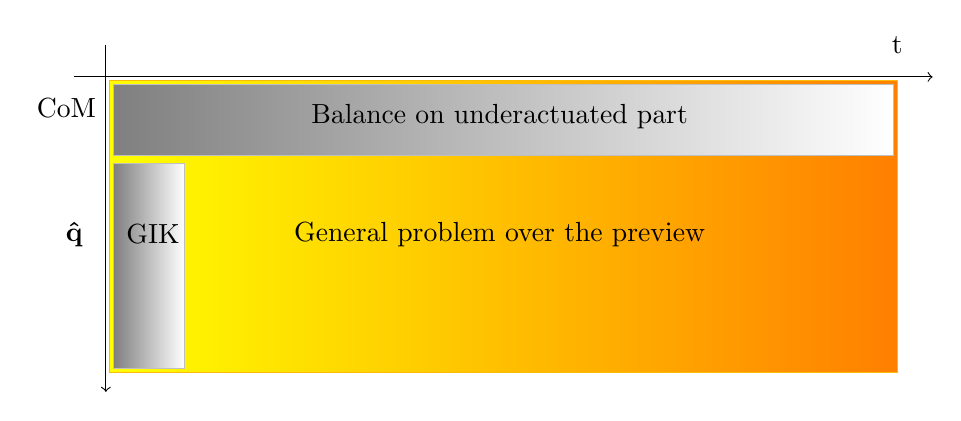
\begin{tikzpicture}
  \draw [->] (-0.4,0) -- (10.5,0);
  \draw [->] (0,0.4) -- (0,-4);
  \shadedraw[left color=yellow, right color= orange, draw=yellow!50!orange](0.05,-0.05) rectangle (10.05,-3.75);
  \shadedraw[left color=gray, right color= white, draw=gray!50!white] (0.1,-0.1) rectangle (10,-1.0);
  \shadedraw[left color=gray, right color= white, draw=gray!50!white](0.1,-1.1) rectangle (1,-3.7);
  \draw (10.05,0.4) node {t};
  \draw (-0.5,-0.4) node {CoM};
  \draw (-0.4,-2.0) node {${\bf \hat{q} }$};
  \draw (5,-0.5) node {Balance on underactuated part};
  \draw (0.6,-2.0) node {GIK};
  \draw (5,-2.0) node {General problem over the preview};
\end{tikzpicture}
\caption{Classical approach (in gray) organization vs. a more global handling of the problem \cite{Todorov:ICRA:2014}}
\label{fig:classical_vs_ddp}
\end{figure}

Fig.~\ref{fig:classical_vs_ddp} depicts the classical approaches used so far.
Indeed the full problem is nonlinear and has around 10 thousand variables and is represented by the whole rectangle.
To be able to solve it researchers used heavy framework for nonlinear optimization.
In fact in \cite{koch:ichr:2014} the authors implemented the above OCP and generated trajectories for the HRP-2 robot.
The software used in this context computes multiple shooting method to solve nonlinear problems.
The solution obtained was a smooth trajectory that allow a HRP-2 robot to step over a $20\,cm$ high obstacle.
The experiment has been done in LAAS-CNRS.
This motion is, for now in LAAS-CNRS, the record in terms of obstacle height.
The bottom heck of this approach is the computation time.
These trajectories took several ours to be computed.
Another formulation implement the complete problem but use simplifications in the contact model.
In \cite{tassa:icra:14} the authors uses Differential Dynamic Programming (DDP) to solve the problem.
This is a very efficient way to compute a solution.
However the current contact model is a spring and damper model.
It produce good enough contact forces to perform multicontact reaching.
However no walking could be performed as the the model provides none dynamically consistent force.
An implementation of this software has been used with HRP-2 in \cite{Koenemann:iros:2015}.
The solver was installed in a remote computer as it still needs multiple powerful CPUs to be used online.
In \cite{Koenemann:iros:2015} the authors used a off board non-real-time Windows
on a $12$-core $4 GHz$ CPU that computes the DDP under $100\,ms$.
The PID controller of the robot runs on an embedded computer using a real time linux with a $2.93\,GHz$ CPU.
The connection between the two computer is done via wifi.

To summarize this, there are not yet powerful techniques that can be used with limited time and computational resources.
As a consequence researchers try to simplify the problem.
The next paragraph presents these approaches.

\subsection*{Mixed formulation}

One simplification consist in taking into account the future of the under-actuated part of the dynamic plus the whole body instantaneous dynamics.
In Fig.~\ref{fig:classical_vs_ddp} this would correspond to the two gray areas but fused together.

During the DARPA robotics challenge the authors of \cite{kuindersma:icra:2014} used a custom active set solver for quadratic programming to solve a mixed formulation.
For the under-actuated formulation they used the seminal work of Kajita \cite{Kajita:icra:2003}.
In addition they used linearized friction cones and optimized the robot joint accelerations.

A recent thesis \cite{phdthesis:sherikov:2016} pursue this work of integrating under-actuated preview control inside a instantaneous whole body controller.
The main difference between Sherikov and Kuindersma's work is the under-actuated model predictive control used.
In fact the walking task of the Sherikov's framework is able to automatically find the foot steps following the formalism of \cite{herdt:iros:2010}.
In Kuindersma's framework the foot steps are precomputed by a planner.

\subsection*{Walking patterns in 3D}

From this subsection on, the hypothesis of separating the under-actuated and whole body motion is made.
The hypothesis is most used in the literature and correspond to the two separated gray rectangles in Fig.~\ref{fig:classical_vs_ddp}.
This means that trajectories for the CoM, the free flyer and the end effectors are computed first.
And only afterward the whole body control is deduced from these preliminary calculations.
The work presented in this section are locomotion algorithm allowing multiple contacts.

An iterative scheme is proposed in \cite{Hirukawa:icra:2007} that can be written as an implicit optimization scheme whose cost function is the distance to a given CoM trajectory and given forces distributions. The resulting forces satisfies \eqref{eq:conic_constraint} by construction of the solution. There is no condition on the angular momentum \eqref{eq:angular:momentum} neither on the viability of the final state \eqref{eq:term_constraint}, however the reference trajectory enforced by the cost function is very likely to play the same role.

In \cite{qiu_dhm11}, \eqref{eq:conic_constraint} is explicitly handled (using the classic linear approximation of the quadratic cones). As in \cite{perrin_isrr15}, \eqref{eq:term_constraint} is indirectly handled by minimizing the jerk. No condition on the angular momentum \eqref{eq:angular:momentum} is considered. Additionally, the proposed cost function maximizes the robustness of the computed forces $\bm\phi$ and minimizes the execution time. Finally, constraints are added to represent the limitation of the robot kinematics.

In \cite{perrin_isrr15}, $\dot \am$ is null by construction of the solution. Moreover, \eqref{eq:conic_constraint} is supposed to always hold by hypothesis and is not checked, while \eqref{eq:term_constraint} is not considered but tends to be enforced by minimizing the norm of the jerk of the CoM, like in \cite{Kajita:icra:2003}. These assumptions result in an (bilinear)-constrained quadratic program that is solved by a dedicated numerical method.

In \cite{rotella_humanoid15}, \eqref{eq:conic_constraint} is handled under a simple closed form solution, while \eqref{eq:term_constraint} is not considered. To stabilize the resolution, the cost function tends to stay close to an initial trajectory of both the CoM and the angular momentum, computed beforehand from a kinematic path. Consequently, \eqref{eq:angular:momentum} is not considered either (as it will simply stay close to the initial guess).

\subsection*{Walking patterns in 2D}
In addition to the previous remarks, another difficulty is the bilinear form of the dynamics \eqref{eq:angulardyn}.
When the contacts are all taken on a same plane, a clever reformulation of the dynamics makes it linear \cite{Kajita:icra:2003}, by neglecting the dynamics of both the CoM altitude and the angular momentum. In that case, \eqref{eq:angulardyn} boils down to the constraint of the center of pressure point (CoP) to be in the support polygon.

Kajita et al. \cite{Kajita:icra:2003} did not explicitly check the constraint \eqref{eq:conic_constraint}.
In exchange, $\ell_u$ is used to keep the control trajectory close to a reference trajectory provided a priori.
Similarly, \eqref{eq:term_constraint} is not checked either.
In exchange, $\ell_x$ tends to stabilize the robot at the end of the trajectory by minimizing the jerk of the CoM.
These three simplifications turns \eqref{eq:ocpgen} into a simple unconstrained problem of linear-quadratic regulation that is implicitly solved by integrating the corresponding Riccati equation.
Interesting motions can be perform using this walking pattern generator.
\cite{evrard2009intercontinental} shows that tele-cooperation was possible using humanoid robot and teh walking pattern generator from \cite{Kajita:icra:2003}.

The LQR was reformulated into an explicit OCP \cite{herdt:ar:2010}, directly solved as quadratic program.
The OCP formulation makes possible the formulation of inequality constraints.
\eqref{eq:conic_constraint} is then explicitly checked under its CoP form.

A modification of this OCP is proposed in \cite{Sherikov:ichr:2014} where \eqref{eq:term_constraint} is nicely approximated by the capturability constraint, which is a linear constraint on the CoM and its first time derivative in case of 2D contacts.

\subsection*{Computing the contact placements}

When considering an explicit OCP formulation, additional static variables can be added to the problem.
Typically, the placement of the contact, that are given as invariant in \eqref{eq:ocpgen}, might be computed at the same time.
This was first proposed in \cite{herdt:ar:2010} for a 2D WPG, and similarly used in \cite{Sherikov:ichr:2014} and other works by the same authors.
Similarly, it was proposed in \cite{rotella_humanoid15} to include it in the proposed 3D WPG, but this feature was not implemented nor demonstrated.
In both cases, the placements of the contacts are unlimited (or similarly limited to a convex compact set).
The problem becomes much harder when the contacts might be taken among a discrete set of placements.
In \cite{deits:ichr:14}, the problem was formulated has a mixed-integer program (i.e. having both continuous and discrete variables) in case of flat contact, and solved using an interior-point solver to handle the discrete constraints.
In \cite{mordatch:tog:12}, the same problem is handled using a dedicated solver relying on a continuation heuristic, and demonstrated for animating the motion of virtual avatars.

This is not an exhaustive bibliography.
Many papers need to be cited but also replaced in their scientific context.
So for sake of clarity, a more detailed bibliography is written at the beginning of each chapter.
This allow a better understanding on the state-of-art which is specific to each chapter of this thesis.


\section*{\koroibot\ Key Performance Indicator (KPI)}
\label{sec:keyperf}

\begin{figure}[ht]
\centering
\includegraphics[angle=90, height=0.2\linewidth]{figures/ground.png}
\includegraphics[height=0.2\linewidth]{figures/beam.png}\\[1ex]
\includegraphics[height=0.2\linewidth]{figures/upstair.png}
\includegraphics[height=0.2\linewidth]{figures/steppingstones.png}
\includegraphics[height=0.2\linewidth]{figures/downstair.png}
\caption{Sample of the experimental setup of the \koroibot\ project in LAAS-CNRS}
\label{fig:koroibot:setupreal}
\end{figure}


In the \koroibot\ project we used key performance indicators (KPI) to analyze the behavior of the robot at the beginning and at the end of the project.
These results lead us toward the improvements to be made.
In 2013 the algorithm mostly used and implemented on HRP-2 in LAAS-CNRS where the walking pattern generators described in \cite{Morisawa:ICRA:2007} and in \cite{herdt:iros:2010}.
The performance indicators chosen were:
\begin{list}{ \arabic{point}.}{%
		\usecounter{point}%
		\setlength{\topsep}{5pt}%
		\setlength{\itemsep}{0pt}%
		\setlength{\parsep}{0pt}%
		\setlength{\labelwidth}{3.em}%
		\setlength{\leftmargin}{2em}%
		\setlength{\labelsep}{0.5em}%
	}

\item[\bluesquare] the execution time $T_M$,
\item[\bluesquare] the time to compute the motion $T_{think}$,
\item[\bluesquare] the total energy consumed during a walking distance $D$,
\begin{equation*}
E_{walk} = \int_{t_b{begin}}^{t_{end}} \tau \omega dt + \int_{t_b{begin}}^{t_{end}} R k_c^2
\tau^2 dt \;,\;\;\; \tilde{E}_{walk} = E_{walk}/D 
\end{equation*}
with $E_{walk}$ being the total energy consumed counting the integral over time of the mechanical power and the electrical power dissipated by the motors. $\tau$ and $\omega$ being respectively the joint torques and velocities, and $R$ with $k_c$ being respectively the motor resistances and torque constants.
\item[\bluesquare] the mechanical energy consumed during a walking distance $D$,
\begin{equation*}
E_{meca} = \int_{t_{begin}}^{t_{end}} \tau \omega dt
 \;,\;\;\; \tilde{E}_{meca} = E_{meca}/D 
\end{equation*}
with $E_{meca}$ being the integral over time of the mechanical power,
\item[\bluesquare] the deviation from the planned trajectory $P_{T_r}$,
\item[\bluesquare] and the maximum speed reached $V_{max}$.
\end{list}
The trajectories were generated offline and repeatedly played on the robot to analyze their robustness.
Samples of the experimental setups can be seen in Fig.~\ref{fig:koroibot:setupreal}.

\subsection*{Straight walking}

\begin{tabular}{|c|c|c|c|c|c|c|c|}
\hline
   $T_M$ & $T_{think}$ & $\tilde{E}_{walk}$ & $\tilde{E}_{meca}$ &
   $P_{T_r}^\theta$ & $P_{T_r}^x$ & $P_{T_r}^y$ & $V_{max}$\\
\hline
   $7\,s$ & $2\,s$ & $47250\,J/m$ & $47070\,J/m$ &
   $-0.0013\,rad$ & $0.026\,m$ & $0.052\,m$ & $0.125\,m/s$\\
\hline
\end{tabular}
\\

From these results we can observe that the HRP-2 is very repeatable.
However the room for improvement lies in the maximum velocity speed which is quiet slow.

\subsection*{3D walking}

Here 3D walking means walking on flat ground but possibly a different height, like stair case or stepping stones.
The walking pattern generators \cite{Morisawa:ICRA:2007,herdt:iros:2010} normally does not allow the possibility to perform movement such as climbing stairs.
For this reason we designed smooth feet 3D trajectories using B-Splines and a prior knowledge of the environment.
Empirically we found trajectories that fits kinematics and dynamics constraints.
The results of these implementation is shown in \cite{naveau:ichr:2014}

\subsection*{Walking in stairs or on stepping stones}

\begin{tabular}{|c|c|c|c|c|c|}
\hline
   $T_M$ & $T_{think}$ & $\tilde{E}_{walk}$ & $\tilde{E}_{meca}$ &
   $P_{T_r}$ & $V_{max}$ \\
\hline
   $7\,s$ & $2\,s$ & $256150,J/m$ & $255270\,J/m$ &
   - & - \\
\hline
\end{tabular}
\\

This results shows the KPI value when the robot goes up the stair case.
The important consumption of energy during the climbing up stairs is to be noted.
Diminishing this power consumption is an important factor as it will decrease the loss of electrical energy and the mechanical stress on the robot.
The repeatability of this experiment is around $40\,\%$.

The results of the KPI, when the robot goes downstairs, are very similar to the going up experiment.
The repeatability of the going down stairs motion is around $95\,\%$.
The only point is that the global energy is twice lower than when the robot is going up.
The reason is that it is less fighting the gravity while going down.

For the stepping stone experiment the KPI were also very similar to the above two experiments.
Though, as expected, the energy consumption is between going up and going down stairs.
The repeatability of this experiment is around $50\,\%$.

\subsection*{Walking on a beam}

The major problem of this experiment is its success rate which is around $20\,\%$.
In order to improve this rate we need to take care of the robot balance and the robot feet placement.
Indeed the two main reasons of the robot fall were the default of balance on the beam and the drift which is important as the beam length is $3\,m$ long.

\subsection*{Step over obstacles}

This manipulation has not been performed in the frame of this thesis.
It is a work published in \cite{koch:ichr:2014} already presented in the above sections.
The improvement to be made here is on the computation time.
As explained before in subsection {"Whole body formulations"}, these trajectory took several hours to be computed.


\section*{Contributions}
\label{section:contribution}

The scientific contributions of my thesis are :
\begin{list}{ \arabic{point}.}{%
		\usecounter{point}%
		\setlength{\topsep}{5pt}%
		\setlength{\itemsep}{0pt}%
		\setlength{\parsep}{0pt}%
		\setlength{\labelwidth}{3.em}%
		\setlength{\leftmargin}{2em}%
		\setlength{\labelsep}{0.5em}%
	}
\item[$\bluesquare$] the design a novel real time walking pattern generator using nonlinear model predictive control (Chap.~\ref{chap:nmpc}),
%The input is a $SE(2)$ velocity $[\dot{x},\dot{y},\dot{\theta}]$. It optimizes simultaneously the position and orientation of the left and right foot respectively.
%The use of a nonlinear solver allow additional functionalities like local obstacle avoidance.
\item[$\bluesquare$] the implementation of two multicontact pattern generators using the centroidal dynamics. They both take the contact placements as input and produce dynamically stable center of mass (CoM) motion (Chap.~\ref{chap:multicontact}).
\end{list}

In the context of the \koroibot\ project several technical contributions are to be noted:
\begin{list}{ \arabic{point}.}{%
		\usecounter{point}%
		\setlength{\topsep}{5pt}%
		\setlength{\itemsep}{0pt}%
		\setlength{\parsep}{0pt}%
		\setlength{\labelwidth}{3.em}%
		\setlength{\leftmargin}{2em}%
		\setlength{\labelsep}{0.5em}%
	}
\item[$\bluesquare$] the integration of a hose manipulation by HRP-2. The robot pick the hose from the floor and pull it to a desired position without falling,
\item[$\bluesquare$] the inclusion of the one third power law as control law for humanoid walking,
\item[$\bluesquare$] the elaboration of transfer rules to use upper body human motions integrated with a walking pattern generator (Chap.~\ref{chap:primitives}),
\item[$\bluesquare$] the study of potential application for humanoid robots in an industrial environment (Chap.~\ref{chap:univworker}) including,
\begin{list}{ \arabic{point}.}{%
		\usecounter{point}%
		\setlength{\topsep}{5pt}%
		\setlength{\itemsep}{0pt}%
		\setlength{\parsep}{0pt}%
		\setlength{\labelwidth}{3.em}%
		\setlength{\leftmargin}{2em}%
		\setlength{\labelsep}{0.5em}%
	}
	\item[$\bluesquare$] the use of fast planning in order to make HRP-2 walking towards a desired position while avoiding obstacles,
	\item[$\bluesquare$] the integration of visual servoing to track a target position while walking,
  \item[$\bluesquare$] the use of the whole body motion generator (Stack-of-Tasks) to evaluate the kinematic feasibility of screwing motions,
	\item[$\bluesquare$] the design of feet 3D trajectory to allow the robot to climb stairs or go across stepping stones and beams,  
\end{list}
\item[$\bluesquare$] the implementation of the dynamic filter on the LAAS-CNRS HRP-2 (An.~\ref{an:dyn:filter}),
\end{list}


\section*{Publications}

\subsection*{Journal}

\subsubsection*{Accepted}

\begin{itemize}
\item \bibentry{naveau:ral:2016}
\end{itemize}

\subsubsection*{Under revision}

\begin{itemize}
\item \bibentry{mukovskiy:jras:2016}
\item \bibentry{orthey:homotopic:2015}
\end{itemize}

\subsection*{Conference}

\subsubsection*{Published}

\begin{itemize}
\item \bibentry{matan:biorob:2016}
\item \bibentry{carpentier:hal-01203507}
\item \bibentry{kudruss:ichr:2015}
\item \bibentry{naveau:ichr:2014}
\item \bibentry{ostasse:ichr:2014}
\end{itemize}

\subsubsection*{Submitted}

\begin{itemize}
\item \bibentry{ramirez:ichr:2016}
\end{itemize}

\setcounter{secnumdepth}{+3}

\ifdefined\included
\else
\bibliographystyle{StyleThese}
\bibliography{16-thesis-mnaveau-short}
\end{document}
\fi
